\documentclass[a4paper]{article}

\usepackage[portuguese]{babel}
\usepackage[utf8]{inputenc}
\usepackage{indentfirst}
\usepackage{graphicx}
\usepackage{verbatim}
\usepackage{caption}
\usepackage{subcaption}
\usepackage{wrapfig}
\usepackage{ragged2e}
\usepackage{listings}
\usepackage{float}

\begin{document}

\setlength{\textwidth}{16cm}
\setlength{\textheight}{22cm}

\title{\Huge\textbf{Eximo}\linebreak\linebreak\linebreak
\Large\textbf{Relatório Intercalar}\linebreak\linebreak
\linebreak\linebreak

\includegraphics[scale=0.1]{res/feup-logo.png}\linebreak\linebreak
\linebreak\linebreak
\Large{Mestrado Integrado em Engenharia Informática e Computação} \linebreak\linebreak
\Large{Programação em Lógica}\linebreak
}

\author{\textbf{Grupo 04: Eximo}\\
Henrique Manuel Martins Ferrolho -  201202772\\
João Filipe Figueiredo Pereira - 201104203 \\
\linebreak\linebreak \\
 \\ Faculdade de Engenharia da Universidade do Porto \\ Rua Roberto Frias, s\/n, 4200-465 Porto, Portugal \linebreak\linebreak\linebreak
\linebreak\linebreak\vspace{1cm}}

\maketitle
\thispagestyle{empty}

%************************************************************************************************
%************************************************************************************************

\newpage

%Todas as figuras devem ser referidas no texto. %\ref{fig:codigoFigura}
%
%%Exemplo de código para inserção de figuras
%%\begin{figure}[h!]
%%\begin{center}
%%\includegraphics[height=1.5cm,width=1.5cm]{white_piece.png}
%%\caption{Peça Branca - Jogador 1}
%%\label{fig:1}
%%\end{center}
%%\end{figure}
%%\includegraphics[scale=0.5]{path relativo da imagem}
%%\includegraphics[scale=•]{•} relativo da imagem}

%%\begin{figure}[h!]
%%\centering
%%\includegraphics[height=1.5cm,width=1.5cm]{white_piece.png}
%%\caption{Peça Branca}
%%\label{fig:whitePiece}
%%\end{figure}

%%\hfill

%%\begin{figure}[h!]
%%\centering
%%
\includegraphics[height=1.5cm,width=1.5cm]{black_piece.png}
%%\caption{Peça Preta}
%%\label{fig:blackPiece}
%%\end{figure}

%%\hfill

%%\begin{figure}[h!]
%%\centering
%%\includegraphics[height=3cm,width=3cm]{board.png}
%%\caption{Tabuleiro}
%%\label{fig:board}
%%\end{figure}




%
%
%\textit{Para escrever em itálico}
%\textbf{Para escrever em negrito}
%Para escrever em letra normal
%``Para escrever texto entre aspas''
%
%Para fazer parágrafo, deixar uma linha em branco.
%
%Como fazer bullet points:
%\begin{itemize}
	%\item Item1
	%\item Item2
%\end{itemize}
%
%Como enumerar itens:
%\begin{enumerate}
	%\item Item 1
	%\item Item 2
%\end{enumerate}
%
%\begin{quote}``Isto é uma citação''\end{quote}

\newpage

%%%%%%%%%%%%%%%%%%%%%%%%%%
\section{O Jogo Eximo}
%%Descrever detalhadamente o jogo, a sua história e, principalmente, as suas regras.
%%Devem ser incluidas imagens apropriadas para explicar o funcionamento do jogo.
%%Devem ser incluidas as fontes de informação (e.g. URLs em rodapé).

\large{\textbf{História}}
\begin{small}

Eximo é um jogo da família das Damas, concebido em 1 de Fevereiro de 2013.\newline
\end{small}

\large{\textbf{Detalhes do Jogo}}
\begin{small}

O jogo realiza-se num tabuleiro 8x8, em que as casas têm todas cores semelhantes. Cada jogador começa com 16 peças colocadas em locais pré-definidos no respectivo lado do tabuleiro. Como mostra a imagem abaixo.\newline

\begin{figure}[h!]
  \begin{minipage}[h!]{0.2\textwidth}
    \includegraphics[width=0.4\textwidth]{res/white_piece.png}
    \centering
    \caption{Peça branca}
    \label{fig:2}
  \end{minipage}
	\quad\quad\quad
  \begin{minipage}[h!]{0.2\textwidth}
    \includegraphics[width=\textwidth]{res/board.png}
    \caption{Tabuleiro}
    \label{fig:3}
  \end{minipage}
	\quad\quad\quad
  \begin{minipage}[h!]{0.2\textwidth}
    
\includegraphics[width=0.4\textwidth]{res/black_piece.png}
	\centering
    \caption{Peça preta}
    \label{fig:4}
  \end{minipage}
\end{figure}

Existe movimento e captura ortogonal e diagonal. Diferente das Damas, não há Dama, apenas homens. Os homens podem saltar sem efectuar captura. Quando um homem atinge a última linha, dá-se a libertação de outro homem.
\end{small}\newline

\large{\textbf{Objetivo}}
\begin{small}

O objetivo do jogo é, assim como nas Damas, \textbf{capturar todas as peças} do oponente, saltando sobre elas, ou \textbf{incapacitar o adversário} de realizar mais algum movimento.
\end{small}\newline

\large{\textbf{Jogada}}
\begin{small}

Em cada jogada, um jogador pode fazer uma de duas ações: \textbf{mover ou capturar}.
\end{small}\newline

\large{\textbf{Movimento}}
\begin{small}

Uma peça pode mover-se em três direções: para frente ou na diagonal (\textbf{norte, nordeste ou noroeste}). Numa jogada, o movimento nunca pode ser efetuado para a retaguarda. 

Existem dois tipos de movimentos: \textbf{Normal e Salto}. 
\begin{itemize}
\item \textbf{Movimento Normal}:
uma peça move-se para um \textbf{quadrado adjacente e vazio}. 
\item \textbf{Movimento em Salto}:
\textbf{uma peça salta sobre uma peça aliada adjacente, se e só se o quadrado correspondente} (ao lado da peça aliada) \textbf{estiver vazio}, colocando assim a peça nesse quadrado. Se a mesma peça do jogador puder continuar a realizar o mesmo movimento de salto sobre outra peça amigavél então pode fazê-lo. \textbf{Durante o movimento de salto a peça não pode capturar peças inimigas}.

Quando existe \textbf{mais de uma maneira} (peça) de \textbf{saltar}, o jogador \textbf{pode escolher qual a peça para executar o salto}, qual o tipo de salto ou sequência de saltos a fazer. A sequência de saltos escolhida pelo jogador não implica a que requere o número máximos de saltos a fazer, porém \textbf{o jogador após escolher uma sequência deve executar todos os saltos nela contida}.
\end{itemize}
\end{small}\pagebreak

\begin{figure}
  \begin{minipage}[b]{0.3\textwidth}
    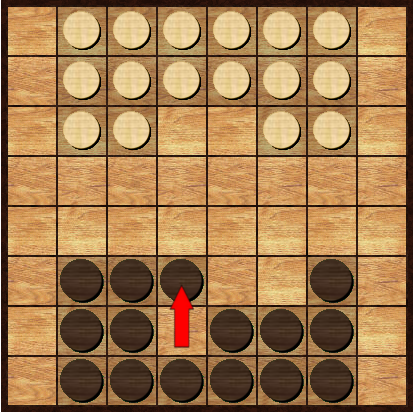
\includegraphics[width=\textwidth]{res/normalMove.png}
    \caption{Movimento Normal}
    \label{fig:5}
  \end{minipage}
\quad\quad\quad\quad\quad\quad\quad\quad
  \begin{minipage}[b]{0.3\textwidth}
    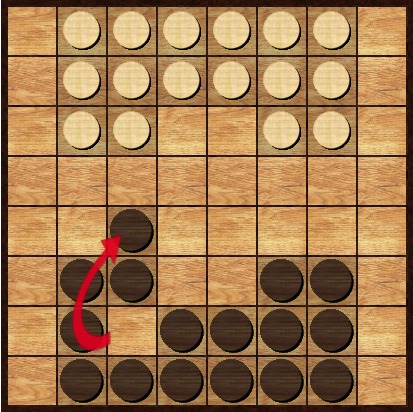
\includegraphics[width=\textwidth]{res/jumpMove.png}
    \caption{Movimento em Salto}
    \label{fig:6}
  \end{minipage}
  \caption{Movimentos}
\end{figure}

\large{\textbf{Captura}}
\begin{small}

Um \textbf{jogador pode capturar} em cinco direções: \textbf{frente}, \textbf{diagonal} (direira ou esquerda), à \textbf{direita} ou à \textbf{esquerda} (norte, nordeste, noroeste, leste ou oeste). 

\begin{itemize}
\item \textbf{Captura}:
um jogador \textbf{salta sobre uma peça adjacente do adversário}, se o \textbf{próximo quadrado} (à peça inimiga), na mesma direção, \textbf{estiver vazio}, colocando, assim, a peça sobre o quadrado vazio. A \textbf{peça do oponente é removida do tabuleiro}. Se a \textbf{peça} do mesmo jogador \textbf{poder continuar a capturar outras peças do adversário} então \textbf{deve fazê-lo}. A \textbf{captura é obrigatória}, e deve continuar enquanto for possível.
\end{itemize}

\begin{figure}[h!]
	\centering
    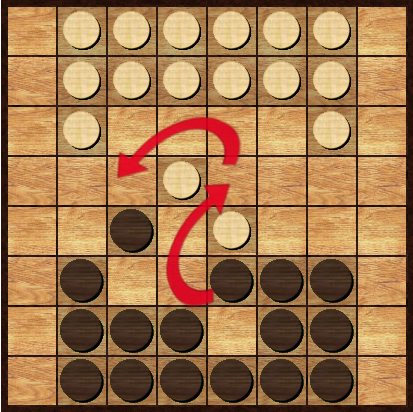
\includegraphics[height=5cm,width=5cm]{res/captureMove.png}
    \caption{Captura}
    \label{fig:7}
\end{figure}

Tal como no \textbf{Movimento de Salto}, \textbf{o jogador escolhe} livremente \textbf{qual sequência de salto a tomar}.
\end{small}\newline

\large{\textbf{Última Linha}}
\begin{small}

Quando uma peça atinge a outra extremidade do tabuleiro, ela, de imediato, é removida do tabuleiro e o jogador recebe dois movimentos extra- TODO Acabar isto, informar sobre as regras
\end{small}\newline

%%%%%%%%%%%%%%%%%%%%%%%%%%
\section{Representação do Estado do Jogo}

%Descrever a forma de representação do estado do tabuleiro (tipicamente uma lista de %listas), com exemplificação em Prolog de posições iniciais do jogo, posições %intermédias e finais, acompanhadas de imagens ilustrativas.

\begin{small}
\begin{lstlisting}
createSeparatorN(0, _, []).
createSeparatorN(N, SS, [SS | Ls]):-
	N1 is N-1,
	createSeparatorN(N1, SS, Ls).
\end{lstlisting}
\end{small}


%%%%%%%%%%%%%%%%%%%%%%%%%%
\section{Visualização do Tabuleiro}

%Descrever a forma de visualização do tabuleiro em modo de texto e o(s) predicado(s) %Prolog construídos para o efeito.
%Deve ser incluída pelo menos uma imagem correspondente ao output produzido pelo %predicado de visualização.

\large{\textbf{Estado Inicial do Jogo}}

\begin{small}
A representação do jogo Eximo terá uma interface simples. O único meio de visualizar o decorrer do jogo é a partir da consola. Demonstramos como será com a imagem abaixo.
\begin{figure}[h!]
	\centering
    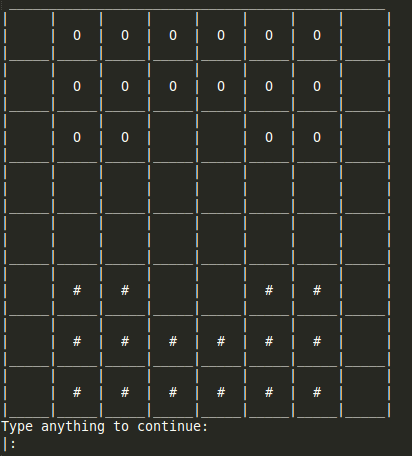
\includegraphics[height=5cm,width=5cm]{res/mazeBoard.png}
    \caption{Tabuleiro na consola}
    \label{fig:8}
\end{figure}
\end{small}\newline

\large{\textbf{Estado Intermédio do Jogo}}

\begin{small}
Como demonstramos em "O Jogo Eximo" os movimentos que o jogador pode fazer, deixamos aqui uma exemplificação do que acontecerá no decorrer de uma partida. A peça que estava inicialmente em \textbf{D7 moveu-se para D8} (Figura 9).
\begin{figure}[h!]
  \begin{minipage}[h!]{0.3\textwidth}
    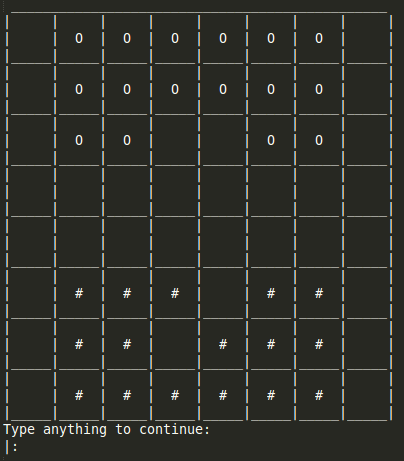
\includegraphics[height=4cm,width=4cm]{res/normalMoveConsole.png}
    \caption{Movimento Normal}
    \label{fig:9}
  \end{minipage}
	\quad\quad\quad\quad	\quad\quad\quad\quad	
  \begin{minipage}[h!]{0.3\textwidth}
    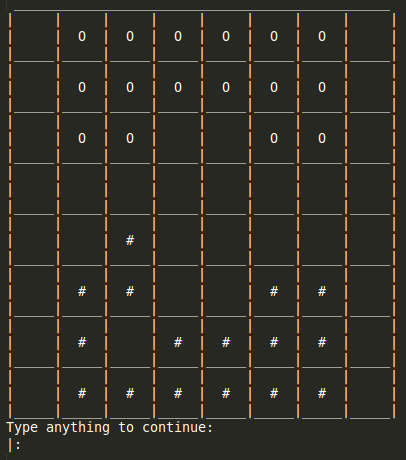
\includegraphics[height=4cm,width=4cm]{res/jumpMoveConsole.png}
    \caption{Movimento Salto}
    \label{fig:10}
  \end{minipage}
\end{figure}\newline
\end{small}

\begin{small}
Quando o jogador quiser realizar o outro tipo de movimento (em salto), deve verificar se o pode ou não realizar, caso contrário, o jogo considerará movimento inválido. Vejamos o caso que também existe em cima na parte de "O Jogo Eximo". O jogador \textbf{executa um salto sobre a peça C4, com a peça C7 e destino C5} (Figura 10). \textbf{Não esquecer que o quadrado destino do salto deve estar vazio}.
\end{small}

%%%%%%%%%%%%%%%%%%%%%%%%%%
\section{Movimentos}

Elencar os movimentos (tipos de jogadas) possíveis e definir os cabeçalhos dos predicados que serão utilizados (ainda não precisam de estar implementados).


\end{document}
